\section{Conclusion}
\label{sec:08:conclusion}

% --- SLIDE 1: GENERAL SUMMARY ---

\begin{frame}{Concluding Remarks: General Summary}
    \begin{block}{A Data-Centric Lightweight Pipeline}
        This work explored a scalable pipeline for parcel-level crop classification using public labels and Sentinel-2 data. The DCAI filtering strategy allowed the creation of datasets even from noisy public sources.
    \end{block}

    \pause

    \begin{block}{Models \& Reliability}
        \begin{itemize}
            \item Deep Learning models generally showed better performance than Shallow baselines, particularly in complex scenarios like Brazil.
            \item Self-Supervised Learning indicated a positive impact as a regularizer in data-scarce regimes.
            \item The proposed \textbf{ORDER} method demonstrated promising potential in separating correct from incorrect predictions, offering a viable alternative to mitigate model overconfidence.
        \end{itemize}
    \end{block}
\end{frame}

% --- SLIDE 2: RQ1 ---

\begin{frame}{Answering RQ1: Data-Centric AI (DCAI)}
    \begin{block}{Research Question 1}
        To what extent can DCAI strategies - specifically, rigorous filtering of noisy public labels - enable the creation of crop classification datasets and improve the performance of crop classification models?
    \end{block}

    \begin{figure}
        \centering
        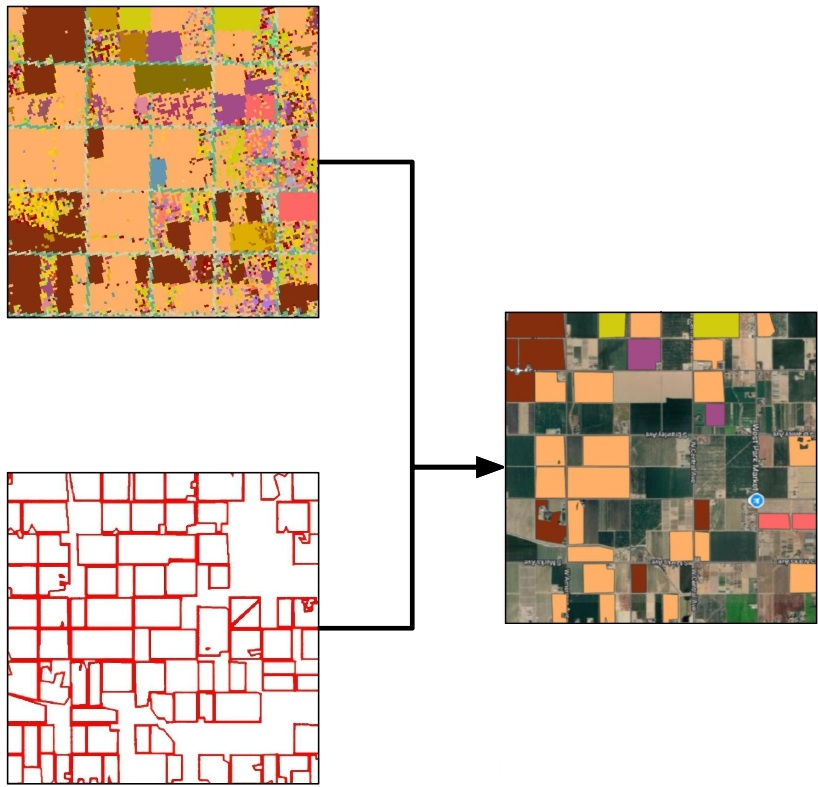
\includegraphics[width=0.4\textwidth, keepaspectratio]{figures_slides/rq1.jpg}
    \end{figure}
\end{frame}

\begin{frame}{Answering RQ1: Data-Centric AI (DCAI)}
    \begin{block}{Research Question 1}
        To what extent can DCAI strategies - specifically, rigorous filtering of noisy public labels - enable the creation of crop classification datasets and improve the performance of crop classification models?
    \end{block}

    \begin{block}{Conclusion}
        \begin{itemize}
            \item The DCAI strategy, combined with public cropland rasters, enables the effective creation of large-scale crop classification datasets.
            \item \textbf{Limitation/Future Work:} To fully isolate and estimate the exact impact of the DCAI performance on downstream models, further studies are necessary, especially focusing on \textbf{actively correcting possible incorrect labels evaluated by the framework}.
        \end{itemize}
    \end{block}
\end{frame}

% --- SLIDE 3: RQ2 ---

\begin{frame}{Answering RQ2: Self-Supervised Learning (SSL)}
    \begin{block}{Research Question 2}
        Do SSL pre-training strategies impact embedding generation and offer a significant advantage over supervised models when labels are scarce? If so, which strategy generates the best embeddings?
    \end{block}

  \begin{figure}
        \centering
        \caption{Few shot (1\%) on Brazil Dataset.}
        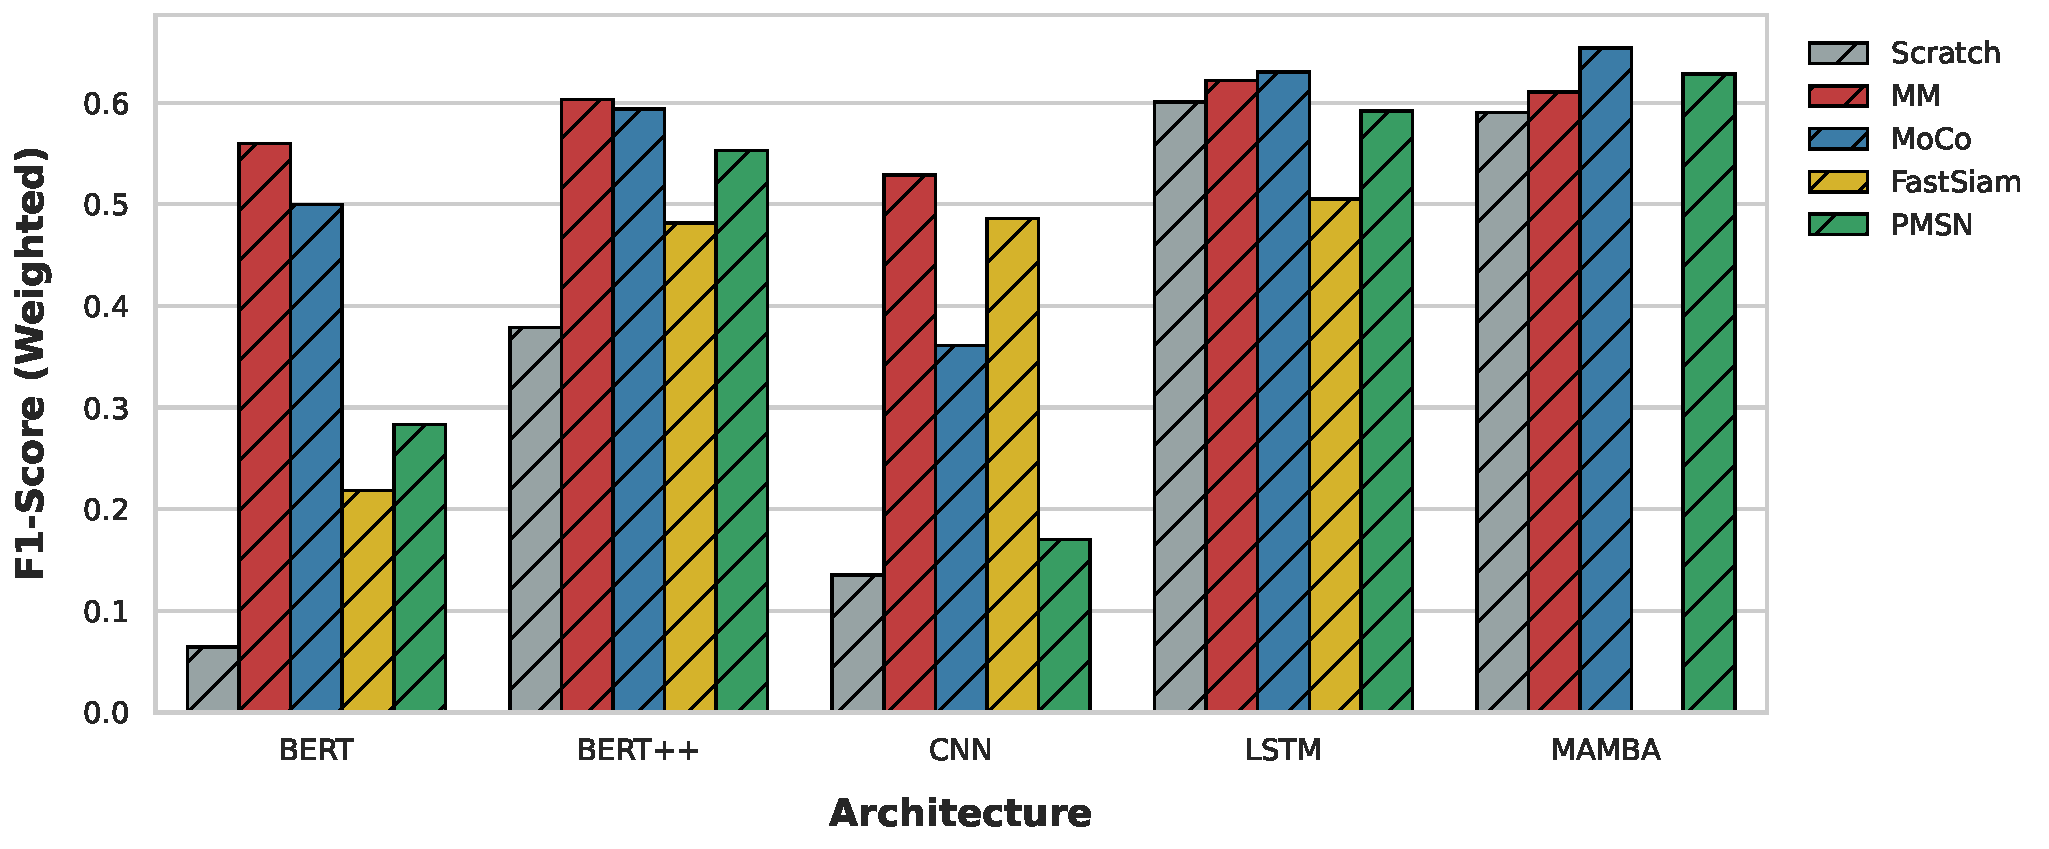
\includegraphics[width=0.8\textwidth, keepaspectratio]{figures/8_results/brazil-finetuning/few_shot_pretraining.pdf}
    \end{figure}
\end{frame}

\begin{frame}{Answering RQ2: Self-Supervised Learning (SSL)}
    \begin{block}{Research Question 2}
        Do SSL pre-training strategies impact embedding generation and offer a significant advantage over supervised models when labels are scarce? If so, which strategy generates the best embeddings?
    \end{block}

    \begin{block}{Conclusion}
        \begin{itemize}
            \item SSL pre-training appears to be a highly effective option for improving classification metrics in label-scarce scenarios (e.g., 1\% and 0.1\% regimes).
            \item Among the evaluated strategies, \textbf{MoCo} stood out, generating consistent metrics in both fine-tuning and direct embedding evaluation (KNN), without presenting severe representation collapse across the experiments.
        \end{itemize}
    \end{block}
\end{frame}

% --- SLIDE 4: RQ3 ---

\begin{frame}{Answering RQ3: Lightweight Pipeline \& Models}
    \begin{block}{Research Question 3}
        Is it possible to build a lightweight pipeline that achieves satisfactory performance for crop classification that can be run without expensive hardware? If so, which models are most suitable?
    \end{block}

  \begin{figure}
        \centering
        %\caption{Few shot (1\%) on Brazil Dataset.}
        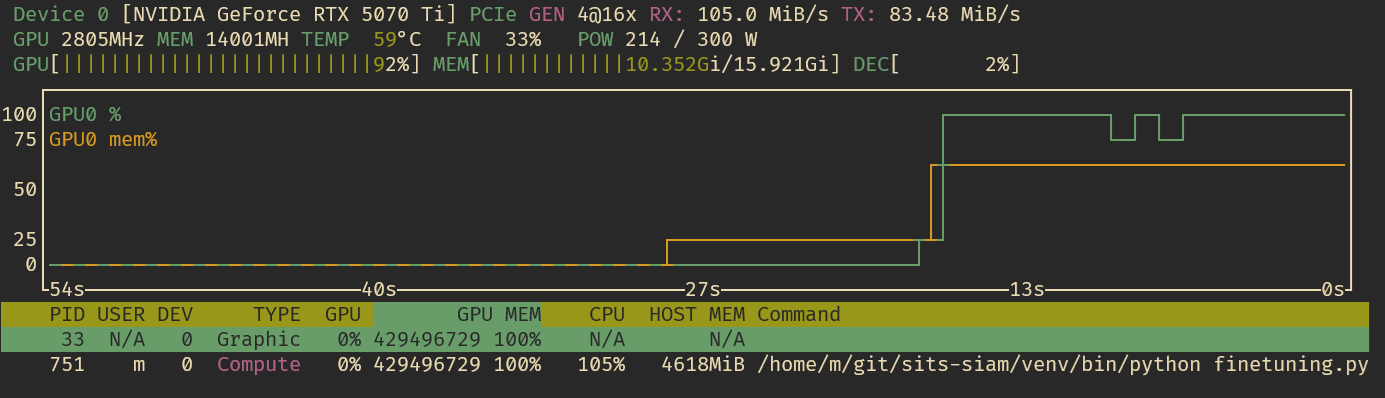
\includegraphics[width=1\textwidth, keepaspectratio]{figures_slides/rq3.png}
    \end{figure}
\end{frame}


\begin{frame}{Answering RQ3: Lightweight Pipeline \& Models}
    \begin{block}{Research Question 3}
        Is it possible to build a lightweight pipeline that achieves satisfactory performance for crop classification that can be run without expensive hardware? If so, which models are most suitable?
    \end{block}

    \begin{block}{Conclusion}
        \begin{itemize}
            \item Yes, the results suggest such a pipeline is feasible. The proposed SITS download method shifts most processing costs to the cloud (GEE), enabling the use of modest local hardware.
            \item \textbf{Suitable Models:} \textbf{SITS-BERT++} yielded slightly higher overall metrics, whereas \textbf{SITS-Mamba} provided a highly balanced trade-off due to its linear processing memory costs, making both strong candidates. All models can be fine-tuned with a modest Nvidia RTX 5070 Ti 16GB.
        \end{itemize}
    \end{block}
\end{frame}

% --- SLIDE 5: RQ4 ---

\begin{frame}{Answering RQ4: Public Sensors Applicability}
    \begin{block}{Research Question 4}
        Is it possible to achieve satisfactory performance for crop classification using only public sensors?
    \end{block}

    \pause

    \begin{block}{Conclusion}
        \begin{itemize}
            \item The experiments indicate that it is indeed possible to generate strong ranking and classification metrics relying exclusively on public missions (such as Sentinel-2).
            \item \textbf{Limitation/Future Work:} To confirm the relative efficiency of this approach, further comparative studies testing these models against private, high-resolution commercial sensors are recommended.
        \end{itemize}
    \end{block}
\end{frame}

% --- SLIDE 6: RQ5 ---

\begin{frame}{Answering RQ5: Anomaly Detection (ORDER)}
    \begin{block}{Research Question 5}
        Is it possible to improve confidence estimation or detect model anomalies through generative models on embeddings, surpassing established baselines such as ConfidNet?
    \end{block}

      \begin{figure}
        \centering
        \caption{Traditional Regime (70\%) on Brazil Dataset, SITS-BERT++ with MoCo.}
        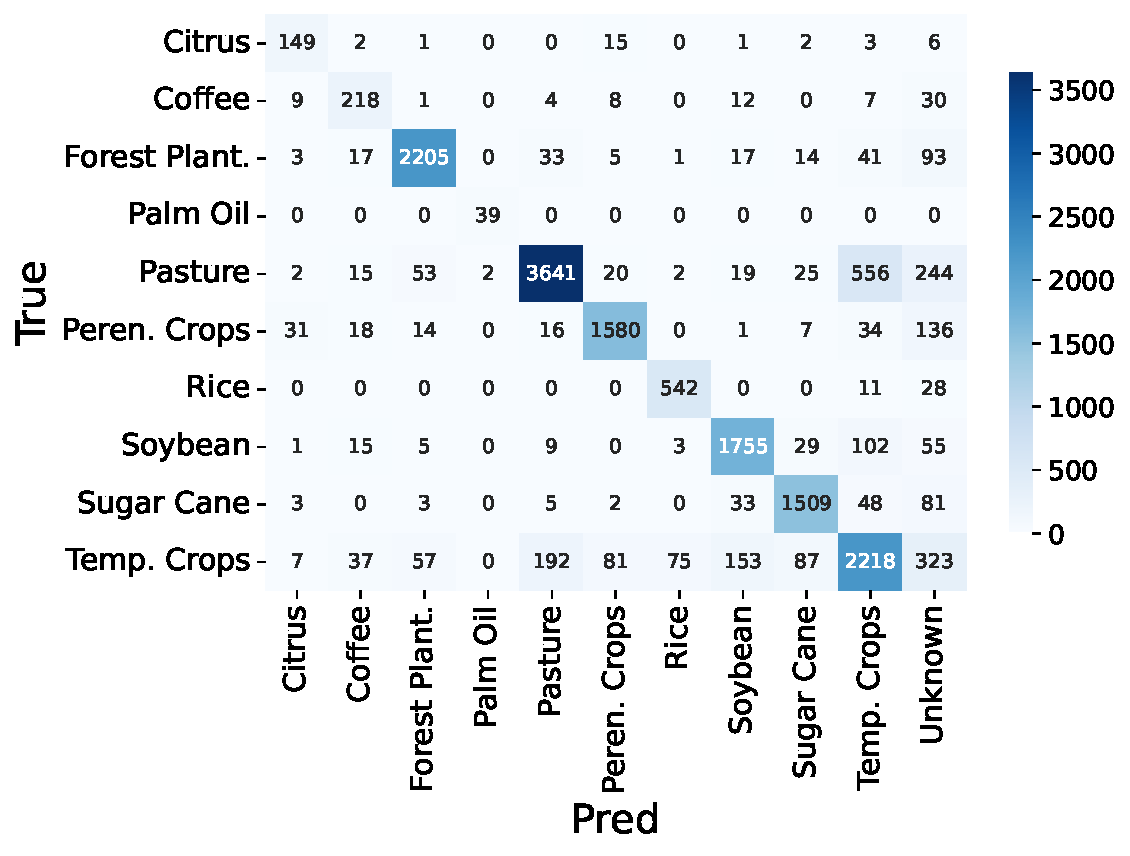
\includegraphics[width=0.4\textwidth, keepaspectratio]{figures/8_results/brazil-finetuning/BERTPP-70.0-MoCo/class_test_gemmos_matrix.pdf}
    \end{figure}
\end{frame}

\begin{frame}{Answering RQ5: Anomaly Detection (ORDER)}
    \begin{block}{Research Question 5}
        Is it possible to improve confidence estimation or detect model anomalies through generative models on embeddings, surpassing established baselines such as ConfidNet?
    \end{block}

    \begin{block}{Conclusion}
        \begin{itemize}
            \item Detecting anomalies during prediction using embedding analysis methods like \textbf{ORDER} proved to be a viable strategy.
            \item \textbf{ORDER} generated a visually clearer bimodal differentiation between correct and incorrect predictions compared to the ConfidNet baseline and the standard Maximum Class Probability (MCP).
            \item While formal confidence ranking was not fully explored, the well-behaved prediction scores suggest it is a promising avenue for future work.
        \end{itemize}
    \end{block}
\end{frame}
